\documentclass{standalone}
\usepackage{pgfplots}
\pgfplotsset{compat=1.18}
\usepgfplotslibrary{fillbetween}

\begin{document}
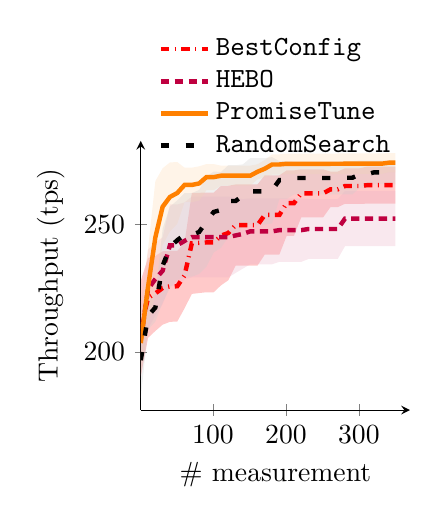
\begin{tikzpicture}
    \begin{axis}[
      axis x line  = bottom,
      axis y line  = left,
      width=5cm, height=5cm, 
      xlabel={\# measurement},
      ylabel={Throughput (tps)},
      xmin=1.0000, xmax=370.0000,
      ymin=177.2032, ymax=282.6294,
      legend cell align=left,
      legend columns=1,
      legend style={
        draw=none, fill=none,
        at={(0.98,0.9)}, anchor=south east,
        legend cell align=left
      }
    ]


\addplot[
    red,
    dashdotted,
    ultra thick, forget plot
] coordinates {
(1.0000, 209.1370) (11.0000, 221.1450) (21.0000, 222.8910) (31.0000, 225.0260) (41.0000, 225.6470) (51.0000, 225.6960) (61.0000, 229.9230) (71.0000, 242.5110) (81.0000, 242.6710) (91.0000, 242.8630) (101.0000, 242.8630) (111.0000, 245.5440) (121.0000, 246.5470) (131.0000, 249.6740) (141.0000, 249.6740) (151.0000, 249.6740) (161.0000, 249.6740) (171.0000, 253.6370) (181.0000, 253.6370) (191.0000, 253.6370) (201.0000, 258.2590) (211.0000, 258.2590) (221.0000, 262.0960) (231.0000, 262.0960) (241.0000, 262.0960) (251.0000, 262.0960) (261.0000, 263.6480) (271.0000, 263.6480) (281.0000, 264.9540) (291.0000, 264.9540) (301.0000, 264.9540) (311.0000, 265.2850) (321.0000, 265.2850) (331.0000, 265.2850) (341.0000, 265.2850) (350.0000, 265.2850)
}; 
\addlegendentry{\texttt{BestConfig}}

\addplot[
name path=upper0,
draw=none, forget plot
] coordinates {
(1.0000, 227.9275) (11.0000, 236.7930) (21.0000, 237.6010) (31.0000, 239.3958) (41.0000, 239.5288) (51.0000, 239.5277) (61.0000, 242.7995) (71.0000, 262.3196) (81.0000, 262.3101) (91.0000, 262.3735) (101.0000, 262.3735) (111.0000, 265.0300) (121.0000, 265.0541) (131.0000, 265.5733) (141.0000, 265.5733) (151.0000, 265.5733) (161.0000, 265.5733) (171.0000, 269.1604) (181.0000, 269.1604) (191.0000, 269.1604) (201.0000, 271.0829) (211.0000, 271.0829) (221.0000, 271.5096) (231.0000, 271.5096) (241.0000, 271.5096) (251.0000, 271.5096) (261.0000, 270.6148) (271.0000, 270.6148) (281.0000, 271.9112) (291.0000, 271.9112) (301.0000, 271.9112) (311.0000, 272.5456) (321.0000, 272.5456) (331.0000, 272.5456) (341.0000, 272.5456) (350.0000, 272.5456)
}; 

\addplot[
name path=lower0,
draw=none, forget plot
] coordinates {
(1.0000, 190.3465) (11.0000, 205.4970) (21.0000, 208.1810) (31.0000, 210.6562) (41.0000, 211.7652) (51.0000, 211.8643) (61.0000, 217.0465) (71.0000, 222.7024) (81.0000, 223.0319) (91.0000, 223.3525) (101.0000, 223.3525) (111.0000, 226.0580) (121.0000, 228.0399) (131.0000, 233.7747) (141.0000, 233.7747) (151.0000, 233.7747) (161.0000, 233.7747) (171.0000, 238.1136) (181.0000, 238.1136) (191.0000, 238.1136) (201.0000, 245.4351) (211.0000, 245.4351) (221.0000, 252.6824) (231.0000, 252.6824) (241.0000, 252.6824) (251.0000, 252.6824) (261.0000, 256.6812) (271.0000, 256.6812) (281.0000, 257.9968) (291.0000, 257.9968) (301.0000, 257.9968) (311.0000, 258.0244) (321.0000, 258.0244) (331.0000, 258.0244) (341.0000, 258.0244) (350.0000, 258.0244)
}; 

% ========= file shading =========
\addplot[
    red!70,
    fill opacity=0.30, forget plot
] fill between[
    of=upper0 and lower0,
];


\addplot[
    purple,
    densely dashed,
    ultra thick, forget plot
] coordinates {
(1.0000, 204.8040) (11.0000, 224.5720) (21.0000, 228.5290) (31.0000, 231.7840) (41.0000, 241.7210) (51.0000, 241.7210) (61.0000, 243.4690) (71.0000, 244.9710) (81.0000, 244.9710) (91.0000, 244.9710) (101.0000, 244.9710) (111.0000, 244.9710) (121.0000, 244.9710) (131.0000, 245.6010) (141.0000, 246.2190) (151.0000, 247.2020) (161.0000, 247.2020) (171.0000, 247.2020) (181.0000, 247.2020) (191.0000, 247.6800) (201.0000, 247.6800) (211.0000, 247.6800) (221.0000, 247.6800) (231.0000, 248.1230) (241.0000, 248.1230) (251.0000, 248.1230) (261.0000, 248.1230) (271.0000, 248.1230) (281.0000, 252.1930) (291.0000, 252.1930) (301.0000, 252.1930) (311.0000, 252.1930) (321.0000, 252.1930) (331.0000, 252.1930) (341.0000, 252.1930) (350.0000, 252.1930)
}; 
\addlegendentry{\texttt{HEBO}}

\addplot[
name path=upper1,
draw=none, forget plot
] coordinates {
(1.0000, 219.2235) (11.0000, 240.0998) (21.0000, 242.7862) (31.0000, 244.8475) (41.0000, 257.7308) (51.0000, 257.7308) (61.0000, 258.5376) (71.0000, 260.8093) (81.0000, 260.8093) (91.0000, 260.8093) (101.0000, 260.8093) (111.0000, 260.8093) (121.0000, 260.8093) (131.0000, 260.2864) (141.0000, 259.8222) (151.0000, 260.1061) (161.0000, 260.1061) (171.0000, 260.1061) (181.0000, 260.1061) (191.0000, 260.1086) (201.0000, 260.1086) (211.0000, 260.1086) (221.0000, 260.1086) (231.0000, 259.8654) (241.0000, 259.8654) (251.0000, 259.8654) (261.0000, 259.8654) (271.0000, 259.8654) (281.0000, 262.9824) (291.0000, 262.9824) (301.0000, 262.9824) (311.0000, 262.9824) (321.0000, 262.9824) (331.0000, 262.9824) (341.0000, 262.9824) (350.0000, 262.9824)
}; 

\addplot[
name path=lower1,
draw=none, forget plot
] coordinates {
(1.0000, 190.3845) (11.0000, 209.0442) (21.0000, 214.2718) (31.0000, 218.7205) (41.0000, 225.7112) (51.0000, 225.7112) (61.0000, 228.4004) (71.0000, 229.1327) (81.0000, 229.1327) (91.0000, 229.1327) (101.0000, 229.1327) (111.0000, 229.1327) (121.0000, 229.1327) (131.0000, 230.9156) (141.0000, 232.6158) (151.0000, 234.2979) (161.0000, 234.2979) (171.0000, 234.2979) (181.0000, 234.2979) (191.0000, 235.2514) (201.0000, 235.2514) (211.0000, 235.2514) (221.0000, 235.2514) (231.0000, 236.3806) (241.0000, 236.3806) (251.0000, 236.3806) (261.0000, 236.3806) (271.0000, 236.3806) (281.0000, 241.4036) (291.0000, 241.4036) (301.0000, 241.4036) (311.0000, 241.4036) (321.0000, 241.4036) (331.0000, 241.4036) (341.0000, 241.4036) (350.0000, 241.4036)
}; 

% ========= file shading =========
\addplot[
    purple!30,
    fill opacity=0.30, forget plot
] fill between[
    of=upper1 and lower1,
];


\addplot[
    orange,
    solid,
    ultra thick, forget plot
] coordinates {
(1.0000, 203.4430) (11.0000, 225.5270) (21.0000, 244.8650) (31.0000, 256.8550) (41.0000, 260.6790) (51.0000, 262.2280) (61.0000, 265.3790) (71.0000, 265.3790) (81.0000, 265.9730) (91.0000, 268.4360) (101.0000, 268.4360) (111.0000, 269.0040) (121.0000, 269.0040) (131.0000, 269.0040) (141.0000, 269.0040) (151.0000, 269.0040) (161.0000, 270.5310) (171.0000, 271.7420) (181.0000, 273.3980) (191.0000, 273.3980) (201.0000, 273.6680) (211.0000, 273.6680) (221.0000, 273.6680) (231.0000, 273.6680) (241.0000, 273.6680) (251.0000, 273.6680) (261.0000, 273.6680) (271.0000, 273.6730) (281.0000, 273.7030) (291.0000, 273.7030) (301.0000, 273.7030) (311.0000, 273.7030) (321.0000, 273.7030) (331.0000, 273.7030) (341.0000, 274.0900) (350.0000, 274.0900)
}; 
\addlegendentry{\texttt{PromiseTune}}

\addplot[
name path=upper2,
draw=none, forget plot
] coordinates {
(1.0000, 215.8626) (11.0000, 240.3988) (21.0000, 266.9174) (31.0000, 271.9102) (41.0000, 274.1959) (51.0000, 274.3584) (61.0000, 272.1540) (71.0000, 272.1540) (81.0000, 272.6831) (91.0000, 273.5488) (101.0000, 273.5488) (111.0000, 272.9393) (121.0000, 272.9393) (131.0000, 272.9393) (141.0000, 272.9393) (151.0000, 272.9393) (161.0000, 273.4908) (171.0000, 275.1571) (181.0000, 277.3834) (191.0000, 277.3834) (201.0000, 277.6930) (211.0000, 277.6930) (221.0000, 277.6930) (231.0000, 277.6930) (241.0000, 277.6930) (251.0000, 277.6930) (261.0000, 277.6930) (271.0000, 277.6935) (281.0000, 277.7379) (291.0000, 277.7379) (301.0000, 277.7379) (311.0000, 277.7379) (321.0000, 277.7379) (331.0000, 277.7379) (341.0000, 277.8373) (350.0000, 277.8373)
}; 

\addplot[
name path=lower2,
draw=none, forget plot
] coordinates {
(1.0000, 191.0234) (11.0000, 210.6552) (21.0000, 222.8126) (31.0000, 241.7998) (41.0000, 247.1621) (51.0000, 250.0976) (61.0000, 258.6040) (71.0000, 258.6040) (81.0000, 259.2629) (91.0000, 263.3232) (101.0000, 263.3232) (111.0000, 265.0687) (121.0000, 265.0687) (131.0000, 265.0687) (141.0000, 265.0687) (151.0000, 265.0687) (161.0000, 267.5712) (171.0000, 268.3269) (181.0000, 269.4126) (191.0000, 269.4126) (201.0000, 269.6430) (211.0000, 269.6430) (221.0000, 269.6430) (231.0000, 269.6430) (241.0000, 269.6430) (251.0000, 269.6430) (261.0000, 269.6430) (271.0000, 269.6525) (281.0000, 269.6681) (291.0000, 269.6681) (301.0000, 269.6681) (311.0000, 269.6681) (321.0000, 269.6681) (331.0000, 269.6681) (341.0000, 270.3427) (350.0000, 270.3427)
}; 

% ========= file shading =========
\addplot[
    orange!30,
    fill opacity=0.30, forget plot
] fill between[
    of=upper2 and lower2,
];


\addplot[
    black,
    loosely dashed,
    ultra thick, forget plot
] coordinates {
(1.0000, 196.7380) (11.0000, 214.1030) (21.0000, 217.3610) (31.0000, 233.7420) (41.0000, 240.9490) (51.0000, 243.7540) (61.0000, 245.8050) (71.0000, 245.8050) (81.0000, 246.9560) (91.0000, 250.9940) (101.0000, 254.7950) (111.0000, 255.5910) (121.0000, 259.0960) (131.0000, 259.0960) (141.0000, 261.2200) (151.0000, 262.8730) (161.0000, 262.8730) (171.0000, 262.8730) (181.0000, 263.2880) (191.0000, 267.2580) (201.0000, 267.2580) (211.0000, 268.0910) (221.0000, 268.0910) (231.0000, 268.0910) (241.0000, 268.0910) (251.0000, 268.0910) (261.0000, 268.0910) (271.0000, 268.0910) (281.0000, 268.1860) (291.0000, 268.1860) (301.0000, 269.5400) (311.0000, 269.5400) (321.0000, 270.3360) (331.0000, 270.3360) (341.0000, 270.3360) (350.0000, 270.3360)
}; 
\addlegendentry{\texttt{RandomSearch}}

\addplot[
name path=upper3,
draw=none, forget plot
] coordinates {
(1.0000, 211.4807) (11.0000, 219.5237) (21.0000, 222.8636) (31.0000, 248.2083) (41.0000, 256.9109) (51.0000, 259.3095) (61.0000, 262.1420) (71.0000, 262.1420) (81.0000, 263.4194) (91.0000, 268.6606) (101.0000, 270.6428) (111.0000, 270.4205) (121.0000, 273.1149) (131.0000, 273.1149) (141.0000, 273.4372) (151.0000, 275.8599) (161.0000, 275.8599) (171.0000, 275.8599) (181.0000, 276.2904) (191.0000, 274.6862) (201.0000, 274.6862) (211.0000, 274.5193) (221.0000, 274.5193) (231.0000, 274.5193) (241.0000, 274.5193) (251.0000, 274.5193) (261.0000, 274.5193) (271.0000, 274.5193) (281.0000, 274.7109) (291.0000, 274.7109) (301.0000, 274.9074) (311.0000, 274.9074) (321.0000, 274.9285) (331.0000, 274.9285) (341.0000, 274.9285) (350.0000, 274.9285)
}; 

\addplot[
name path=lower3,
draw=none, forget plot
] coordinates {
(1.0000, 181.9953) (11.0000, 208.6823) (21.0000, 211.8584) (31.0000, 219.2757) (41.0000, 224.9871) (51.0000, 228.1985) (61.0000, 229.4680) (71.0000, 229.4680) (81.0000, 230.4926) (91.0000, 233.3274) (101.0000, 238.9472) (111.0000, 240.7615) (121.0000, 245.0771) (131.0000, 245.0771) (141.0000, 249.0028) (151.0000, 249.8861) (161.0000, 249.8861) (171.0000, 249.8861) (181.0000, 250.2856) (191.0000, 259.8298) (201.0000, 259.8298) (211.0000, 261.6627) (221.0000, 261.6627) (231.0000, 261.6627) (241.0000, 261.6627) (251.0000, 261.6627) (261.0000, 261.6627) (271.0000, 261.6627) (281.0000, 261.6611) (291.0000, 261.6611) (301.0000, 264.1726) (311.0000, 264.1726) (321.0000, 265.7435) (331.0000, 265.7435) (341.0000, 265.7435) (350.0000, 265.7435)
}; 

% ========= file shading =========
\addplot[
    black!20,
    fill opacity=0.30, forget plot
] fill between[
    of=upper3 and lower3,
];


\addlegendimage{red, dashdotted, ultra thick}
\addlegendentry{\texttt{BestConfig}}
\addlegendimage{purple, densely dashed, ultra thick}
\addlegendentry{\texttt{HEBO}}
\addlegendimage{orange, solid, ultra thick}
\addlegendentry{\texttt{PromiseTune}}
\addlegendimage{black, loosely dashed, ultra thick}
\addlegendentry{\texttt{RandomSearch}}

\end{axis}
\end{tikzpicture}
\end{document}
